%==============================================
\section{Dimensioning a Tokamak}
%==============================================
From the previous equations mostly derived from a 0-dimensional approach (shaped profiles have not been considered so far), a suitable couple $(R, B)$ may be found for a given reactor project of prescribed $(P_{DT}, Q)$. By proceeding this way, some other characteristics of the plasma (namely the shape of the plasma, including elongation and aspect ratio, the average ion mass $\hat M$, the edge safety factor $q_a$ and the density $n_N$ normalised to the Greenwald density) are assumed to be prescribed by other considerations. Notice however that these other variables actually offer additional degrees of freedom to the exercise. The method is applied to the ITER case in section \ref{sec:ITER_spec}.

Should such a $(R, B)$ couple be found, additional important questions then arise before deciding whether it effectively constitutes a suitable tokamak. These includes, but are not limited to, the issues of superconducting magnets with their cryostat and neutron shielding, the issue of power exhaust and of the maximum affordable heat flux per square meter, the capacity to sustain a sufficiently long a plateau of plasma current...\\

%----------------------------------------------
\subsection{Recovering ITER specifications}
\label{sec:ITER_spec}

The objective here is to find a suitable couple of major radius and magnetic field $(R,B)$ which would allow one to reach the ITER targets in terms of fusion gain $Q=10$ and fusion power $\hat P_{DT}=410$ MW.
So as to get closer to the actual specifications of ITER, one should first refine the various constants introduced in section \ref{sec:governing_eqs}. One introduces the following refinements:
\begin{enumerate}
    \item $f_\alpha \doteq n_{He}/n_e$ the fraction of $\alpha$ particles
    \item $f_p \doteq \langle T^2 \rangle / \langle T \rangle^2$ the peaking factor of the temperature profile (a flat density profile is assumed)
    \item $\theta_i \doteq T_i/T_e$ the ratio of ion to electron temperatures
\end{enumerate}
Several coefficients are modified by these additional variables:
\begin{eqnarray*}
    && C_{fus} \to C_{fus} \times (1-2f_\alpha)^2\theta_i^2 \times f_p \\
    && C_{loss} \to C_{loss} \times \frac{1+\theta_i - f_\alpha\theta_i}{2}  \\
    && C_\beta \to C_\beta \times \frac{1+\theta_i - f_\alpha\theta_i}{2}
\end{eqnarray*}
The corrections regarding $C_{fus}$ result from the fact that $P_{DT}$ scales like $\langle n_Dn_TT_i^2 \rangle$, with $n_D = n_T = 0.5\; (1-2f_\alpha)n_e$ so as to fulfil electro-neutrality ($n_D+n_T+2n_{He}=n_e$), and $\langle T_i^2 \rangle = f_p\; \langle T_i \rangle^2$ by definition. The correction regarding $C_{loss}$ and $C_\beta$ is due to the fact that both the power loss and $\beta$ scale like the total pressure which reads: $\sum_s n_sT_s = n_eT_e (1+\theta_i- f_\alpha \theta_i)$ with the assumption that $T_\alpha=T_i$.

In addition, the effective mass $\hat M$ simply derives from $f_\alpha$\footnote{Indeed, one has: $(n_D+n_T+n_{He})\; \hat M = n_D\hat M_D + n_T\hat M_T + n_{He}\hat M_{He} =
n_e\left\{ (\hat M_D + \hat M_T)(1-2f_\alpha)/2 + f_\alpha \hat M_\alpha \right\}$, with $\hat M_D=2$, $\hat M_T=3$ and $\hat M_\alpha=4$.}:
\begin{equation*}
    \hat M = \frac{5  - 2f_\alpha}{2(1-f_\alpha)}
\end{equation*}

Finally, geometrical effects modify the $C_i$ coefficient. The revised expression reads as follows (cf. eq.(17) in \cite{Johner2011}, taken at vanishing triangularity):
\begin{equation*}
    && C_i \to C_i \times 
    \frac{(1.17-0.65\, \varepsilon)(1+\kappa^2)}{2\;(1-\varepsilon^2)^2}
\end{equation*}


\begin{figure} 
	\begin{center}
		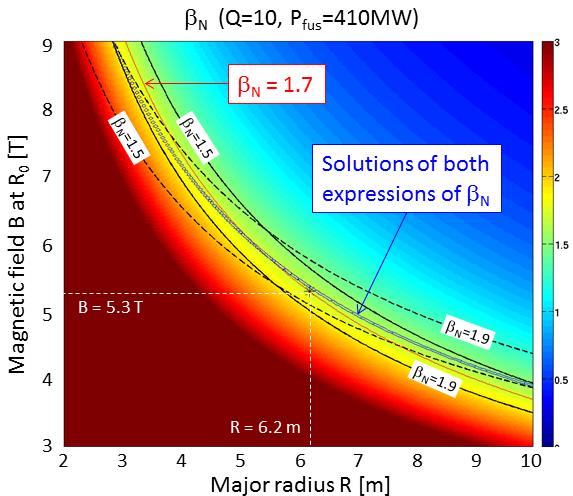
\includegraphics[width=0.75\textwidth]{figures/Fig_2D_betaN_R_B_ITER_ok.png}
		\caption{Map of $\beta_N=f(R,B)$ solutions of eq.\ref{eq:DT_fusion_power_betaN} and eq.\ref{eq:nTtau_betaN}.}
		\label{fig:solutions_betaN}
	\end{center}
\end{figure}

\begin{figure} 
	\begin{center}
		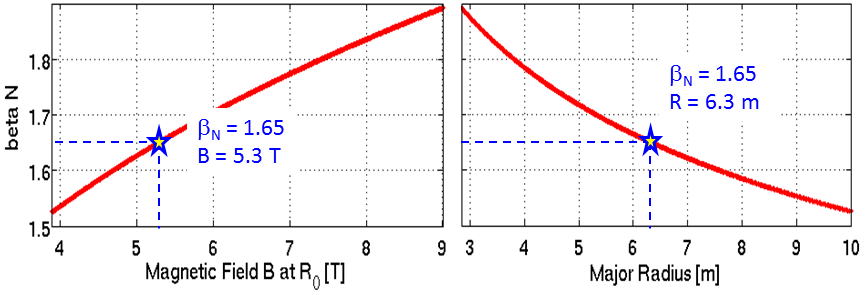
\includegraphics[width=1.\textwidth]{figures/Fig_betaN_solutions_2graphsRB.png}
		\caption{Solution values of $\beta_N$ (taken along the blue line of fig.\ref{fig:solutions_betaN}). The star is close to the ITER specifications in terms of $R$, $B$ and $\beta_N$.}
		\label{fig:}
	\end{center}
\end{figure}
